\documentclass{beamer}

\usepackage{graphicx}
\usepackage{mathtools}
\usepackage{mathrsfs}
\usepackage{fdsymbol}

%Information to be included in the title page:
\title{Multivariate Causal Models}
\author{Congyuan Duan}
%\institute{School of Mathematics, Sun Yat-sen University}



\begin{document}

\frame{\titlepage}

\begin{frame}
    \frametitle{Contents}
    \tableofcontents
\end{frame}

\section{Graph Terminology}

\begin{frame}
    \frametitle{Contents}
    \tableofcontents[currentsection]
\end{frame}

\begin{frame}
    \frametitle{Graph Terminology} 
    \begin{itemize}
        \item[$\bullet$] Consider finitely many random variables $X = (X_1,\cdots,X_d)$ with index set $V=\{1,\cdots,d\}$, 
        joint distribution $P_X$, and density $p(x)$. The corresponding graph is $\mathcal{G} = (V,\mathcal{E})$.
        \item[$\bullet$] We say that there is an \textbf{undirected edge} between two adjacent nodes $i$ and $j$ if 
        $(i,j)\in \mathcal{E}$ and $(j,i)\in \mathcal{E}$. An edge between two adjacent nodes is \textbf{directed} if it is not 
        undirected. We call $\mathcal{G}$ \textbf{directed} if all its edges are directed.
        \item[$\bullet$] Three nodes are called an \textbf{immorality} or a \textbf{v-structure} if one node is a child 
        of the two others that themselves are not adjacent.
        \item[$\bullet$] The \textbf{skeleton} of $\mathcal{G}$ does not take the directions of the edges into account. 
    \end{itemize}
\end{frame}

\begin{frame}
    \frametitle{Graph Terminology}
    \begin{itemize}
        \item[$\bullet$] A \textbf{path} in $\mathcal{G}$ is a sequence of distinct vertices $i_1,\cdots,i_m$, such that
        there is an edge between $i_k$ and $i_{k+1}$ for all $k = 1,\cdots,m-1$. If $i_{k-1}\rightarrow i_k$ and
        $i_{k+1}\rightarrow i_k$, $i_k$ is called a \textbf{collider relative to this path}.
        \item[$\bullet$] All ancestors of $i$ are denoted by $AN_i^{\mathcal{G}}$ and $i$ is not
        an ancestor of itself. We denote all descendants of $i$ by $DE_i^{\mathcal{G}}$ and all non-descendants of $i$,
        excluding $i$, by $ND_i^{\mathcal{G}}$. $ND_i^{\mathcal{G}}$ include the parents of i in graph $\mathcal{G}$.
        \item[$\bullet$] A graph $\mathcal{G}$ is called a \textbf{partially directed acyclic graph (PDAG)} if there is no
        directed cycle, that is, if there is no pair $(j, k)$ with directed paths from $j$ to $k$ and
        from $k$ to $j$. $\mathcal{G}$ is called a \textbf{directed acyclic graph (DAG)} if it is a PDAG and all
        edges are directed.
    \end{itemize}
\end{frame}

\begin{frame}
    \frametitle{Graph Terminology} 
    \centering{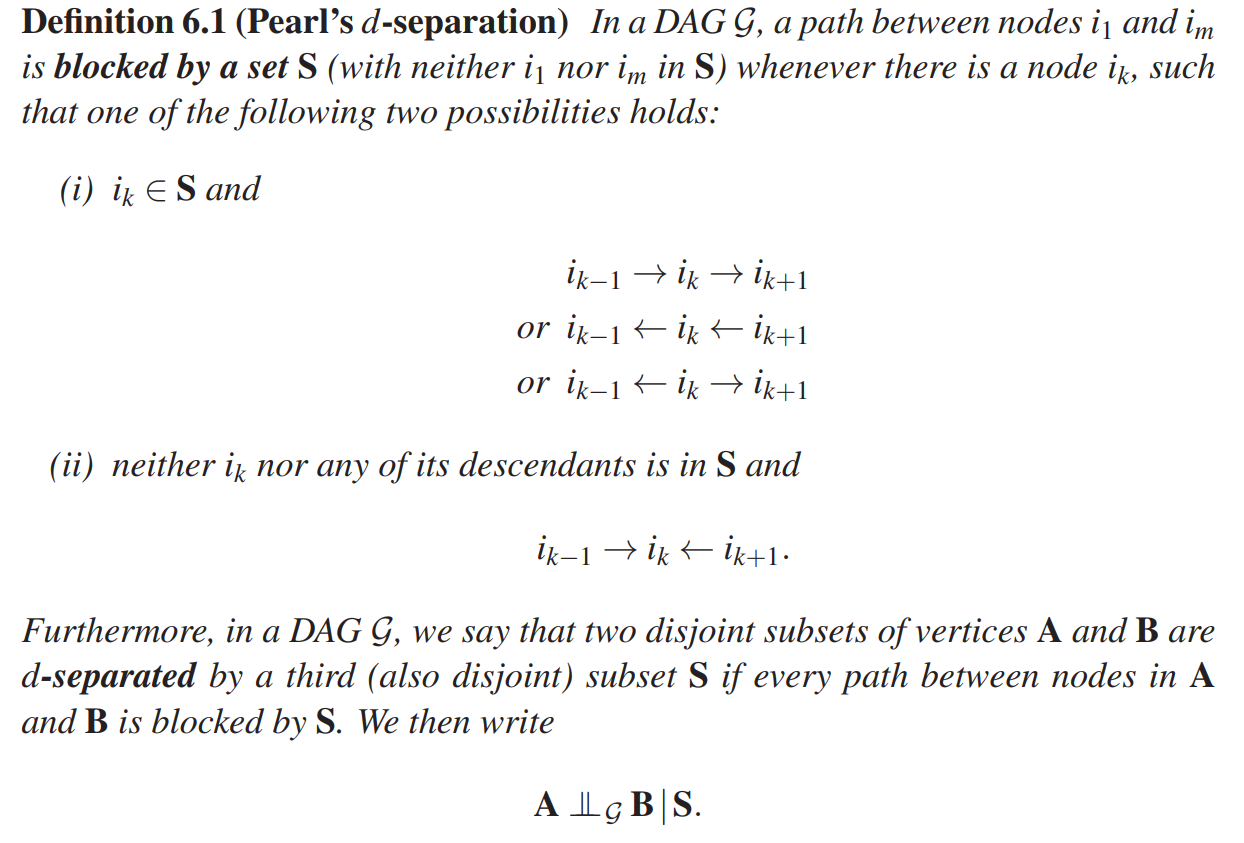
\includegraphics[scale=0.6]{fig1.png}} 
\end{frame}

\begin{frame}
    \frametitle{Example} 
    \centering{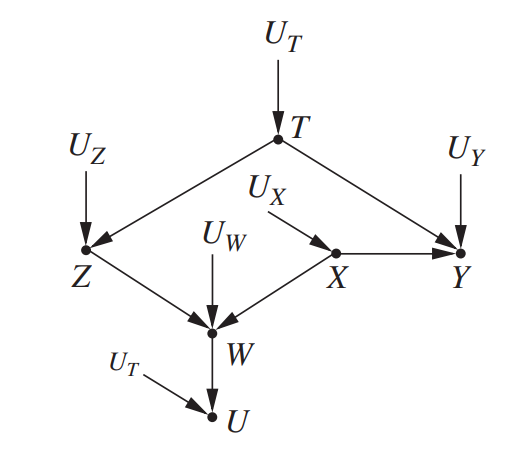
\includegraphics[scale=0.6]{fig41.png}} 
    \begin{itemize}
        \item[$\bullet$] $Z$ and $Y$ are unconditionally dependent
        \item[$\bullet$] Condition on $T$, $Z$ and $Y$ become independent
        \item[$\bullet$] Condition on $\{T, W\}$, $Z$ and $Y$ become dependent
        \item[$\bullet$] Condition on $\{T, W, X\}$, $Z$ and $Y$ become independent again  
    \end{itemize}
\end{frame}


\section{Structural Causal Models}

\begin{frame}
    \frametitle{Contents}
    \tableofcontents[currentsection]
\end{frame}

\begin{frame}
    \frametitle{Definition} 
    \centering{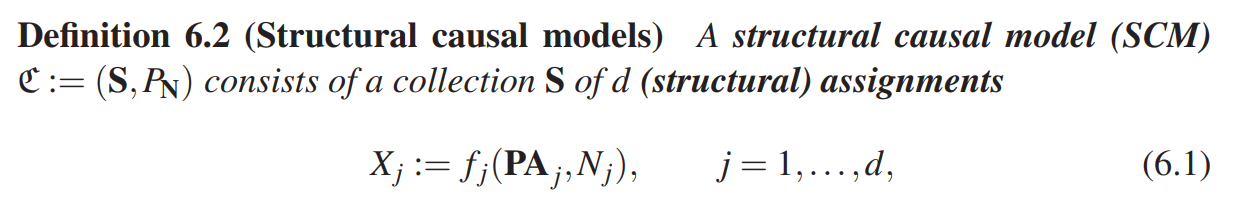
\includegraphics[scale=0.6]{fig2.png}} 
    \centering{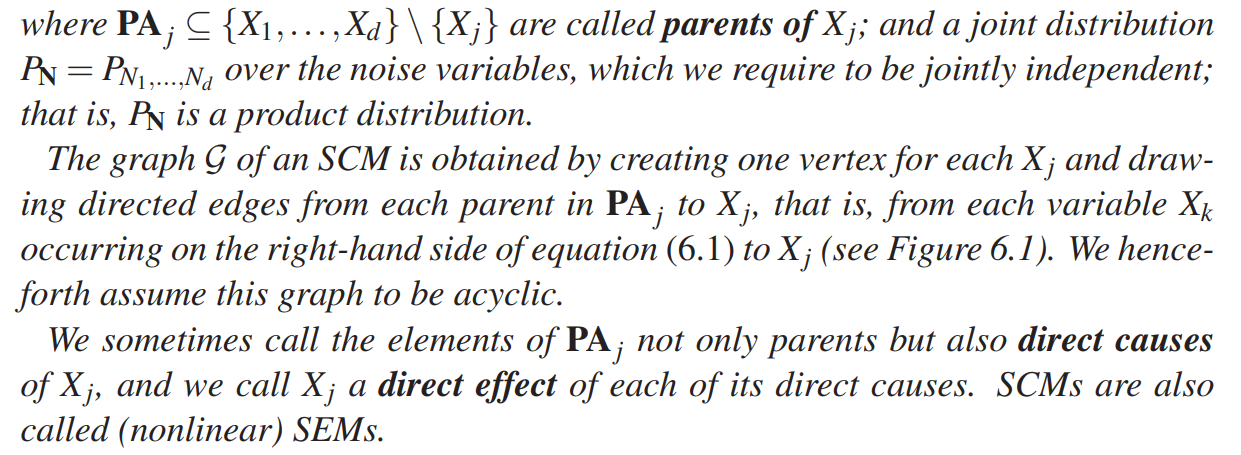
\includegraphics[scale=0.6]{fig3.png}}
\end{frame}

\begin{frame}
    \frametitle{Example} 
    \centering{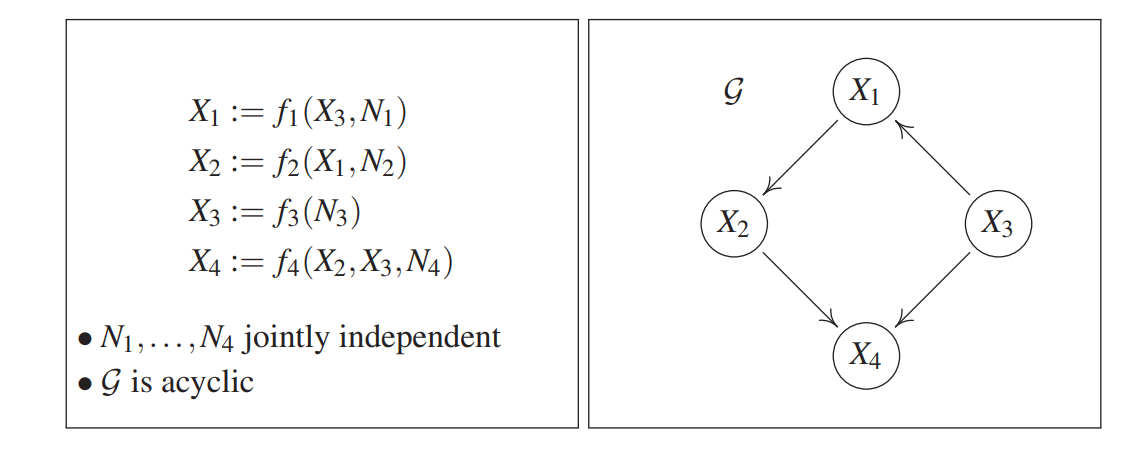
\includegraphics[scale=0.6]{fig5.png}} \\
    \leftline{In this book we focus mainly on acyclic structures.}
\end{frame}

\begin{frame}
    \frametitle{Entailed distributions} 
    \centering{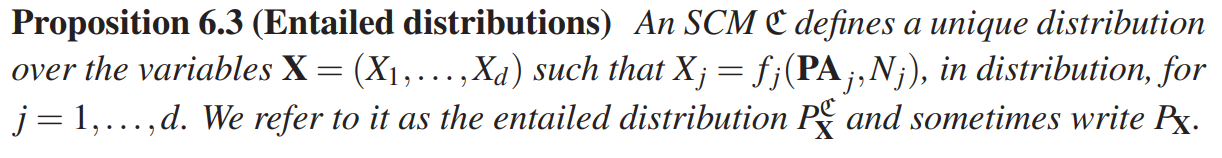
\includegraphics[scale=0.6]{fig6.png}}
    \centering{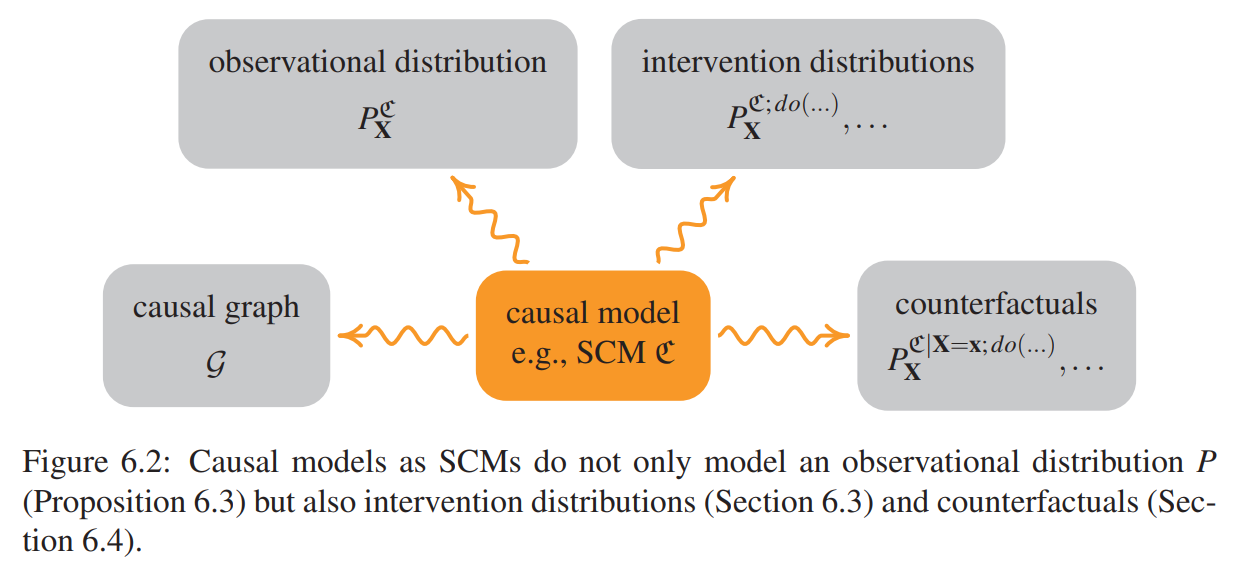
\includegraphics[scale=0.6]{fig7.png}}
\end{frame}

\begin{frame}
    \frametitle{Structural minimality of SCMs} 
    \centering{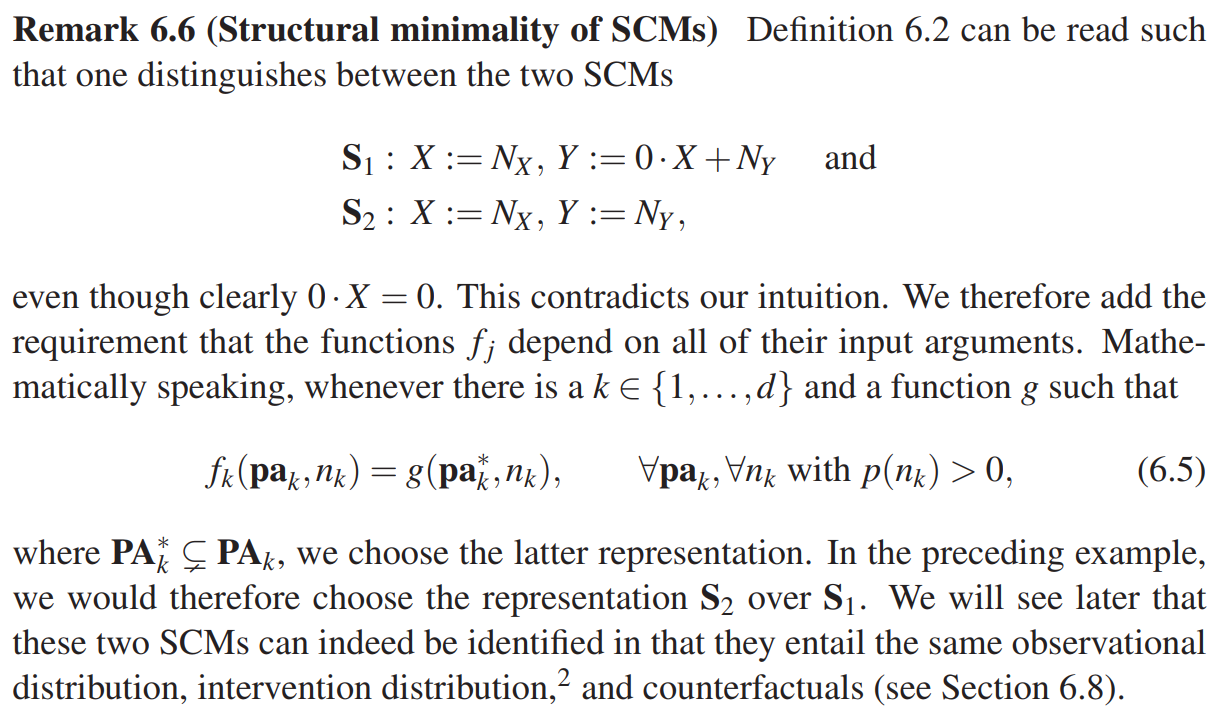
\includegraphics[scale=0.6]{fig8.png}}
\end{frame}

\section{Interventions}

\begin{frame}
    \frametitle{Contents}
    \tableofcontents[currentsection]
\end{frame}

\begin{frame}
    \frametitle{Definition} 
    \centering{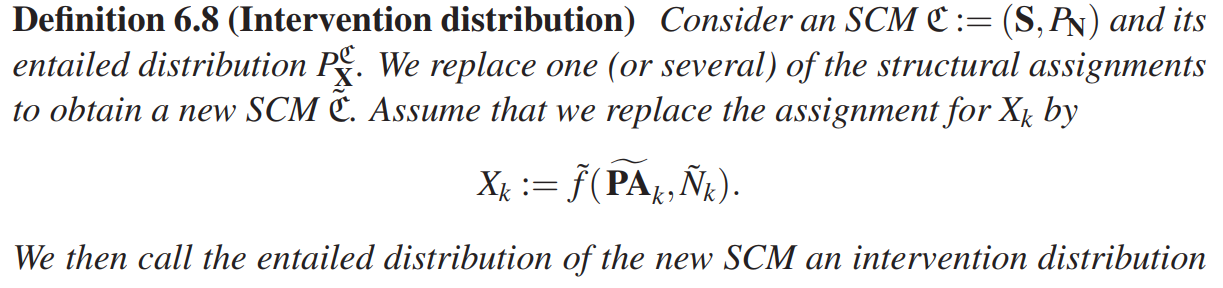
\includegraphics[scale=0.6]{fig9.png}}
    \centering{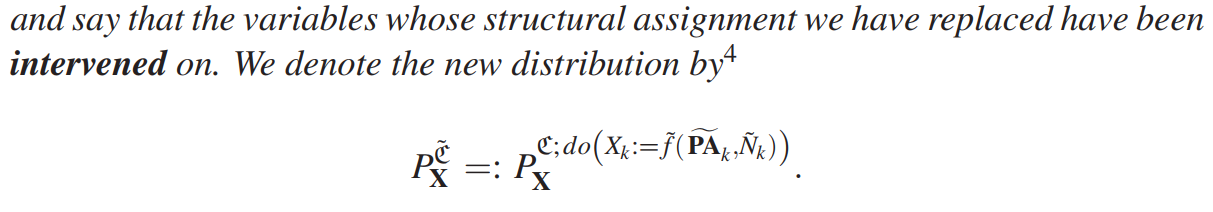
\includegraphics[scale=0.6]{fig10.png}}
    \begin{itemize}
        \item[$\bullet$] The causal parents of the intervened variable have changed. 
        \item[$\bullet$] Intervention distributions differ from the observational distribution.
    \end{itemize}
\end{frame}

\begin{frame}
    \frametitle{Example} 
    \leftline{Consider the SCM} 
    \centering{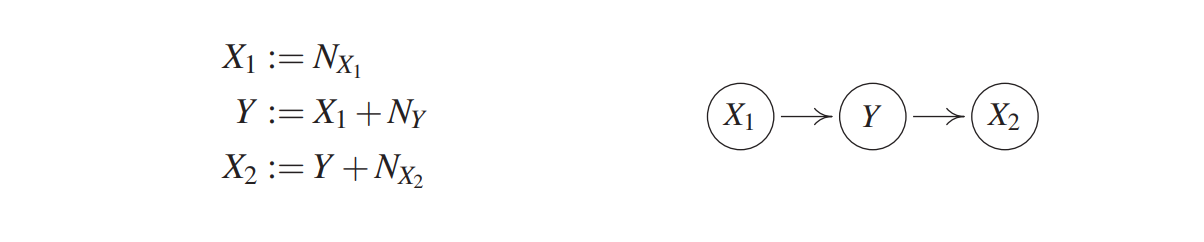
\includegraphics[scale=0.6]{fig11.png}} \\
    \leftline{with $N_{X1},N_Y\sim N(0,1)$ and $N_{X2}\sim N(0,0.1)$.}
    \leftline{Interventions on $X_2$ are useless} 
    \centering{
\includegraphics[scale=0.6]{fig12.png}} \\
    \leftline{Intervention on $X_1$, however, does change the distribution of $Y$} 
    \centering{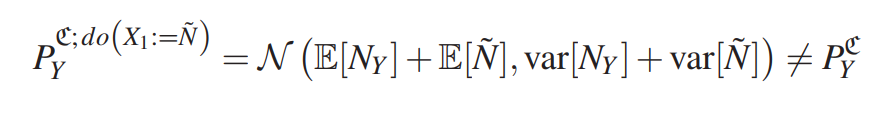
\includegraphics[scale=0.6]{fig13.png}} \\
    \leftline{Intervening is usually different from conditioning} 
    \centering{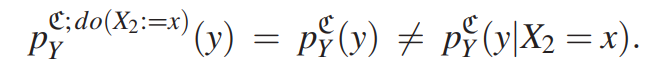
\includegraphics[scale=0.6]{fig14.png}}
\end{frame}

\begin{frame}
    \frametitle{Example: Myopia} 
    \leftline{Assume that the underlying SCM is of the form}
    \centering{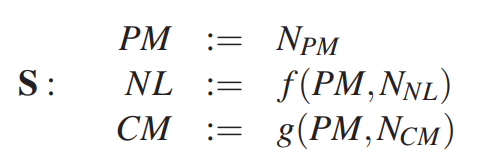
\includegraphics[scale=0.6]{fig15.png}} \\
    \leftline{where PM stands for parent myopia, NL for night light, and CM for}
    \leftline{child myopia.}
    \centering{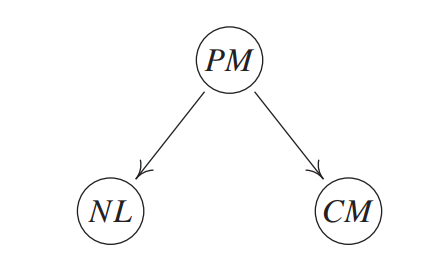
\includegraphics[scale=0.6]{fig16.png}} \\ 
    \begin{flushleft}
        Replacing the structural assignment of NL with $NL := \tilde{N}_{NL}$, where $\tilde{N}_{NL}$ could randomly assign one 
        out of the three night light conditions(darkness, night light, room light) with equal probability, we would find $NL\Vbar CM$.
    \end{flushleft}
\end{frame}

\begin{frame}
    \frametitle{Total causal effects} 
    \centering{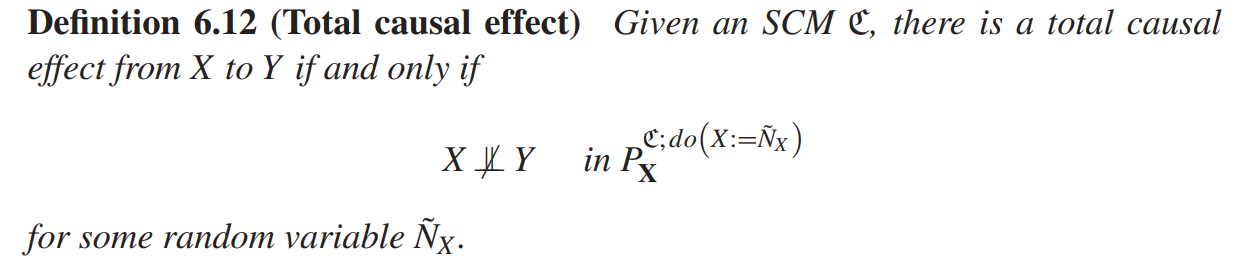
\includegraphics[scale=0.6]{fig17.png}} 
    \centering{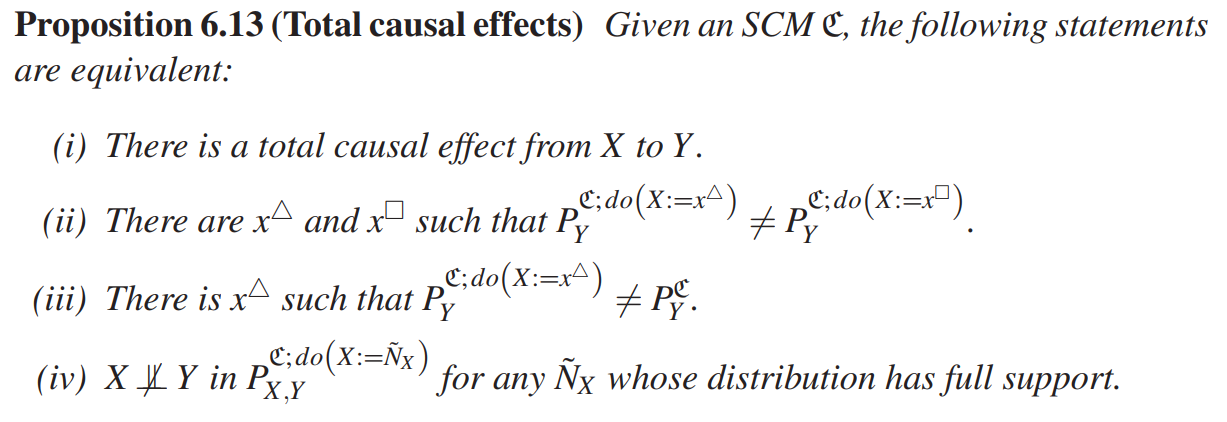
\includegraphics[scale=0.6]{fig18.png}} 
\end{frame}

\begin{frame}
    \frametitle{Total causal effects} 
    \centering{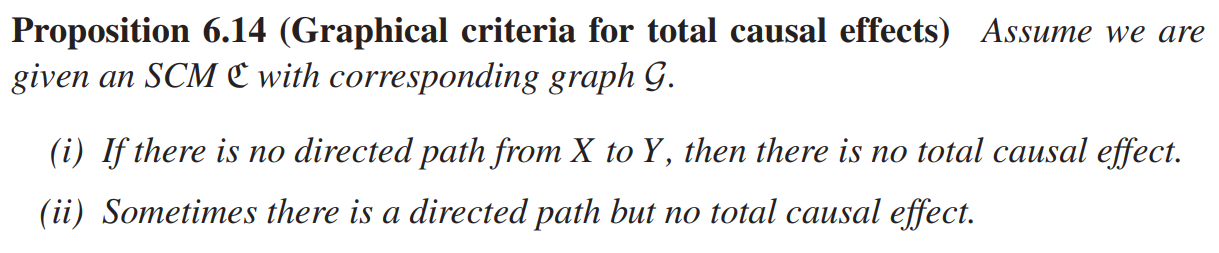
\includegraphics[scale=0.6]{fig19.png}}
\end{frame}

\begin{frame}
    \frametitle{Example: Randomized trials} 
    \centering{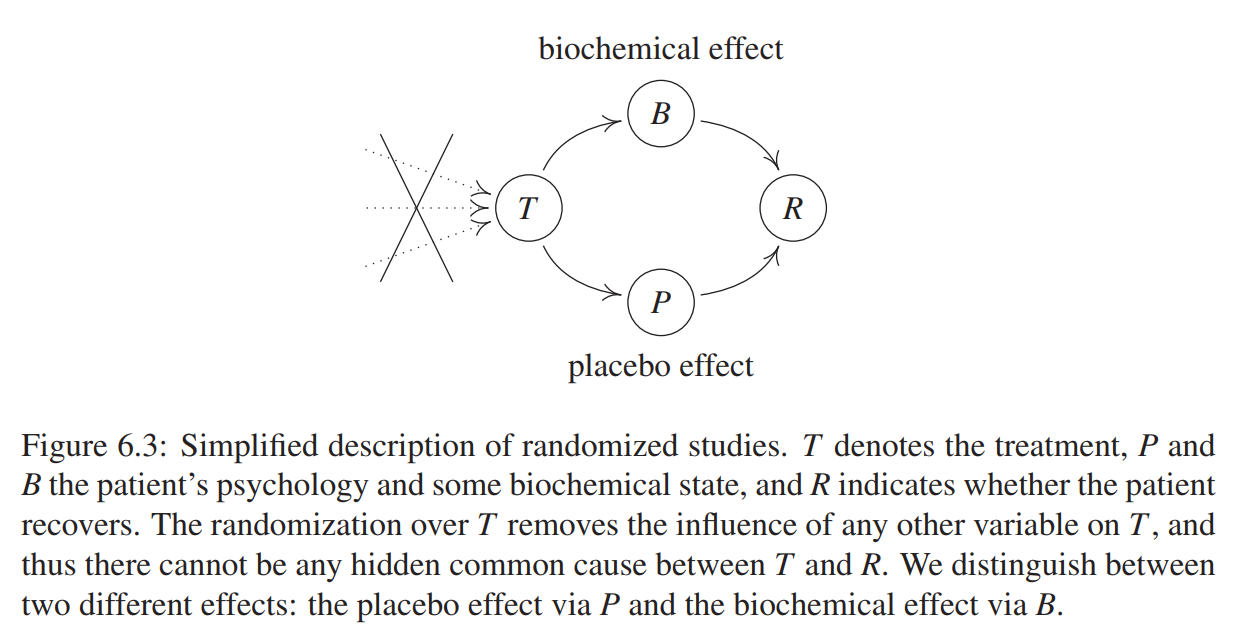
\includegraphics[scale=0.6]{fig20.png}}
    $T = 0$: no medication, $T = 1$: placebo, $T = 2$: drug of interest
\end{frame}

\begin{frame}
    \frametitle{Example: Kidney stones} 
    \centering{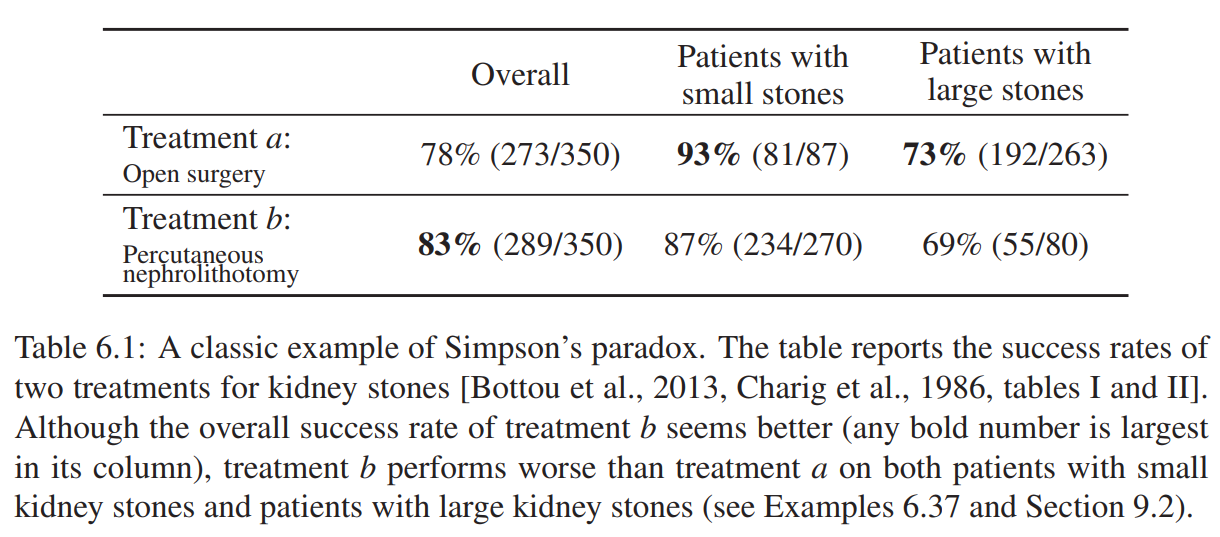
\includegraphics[scale=0.6]{fig21.png}}
\end{frame}


\section{Counterfactuals}

\begin{frame}
    \frametitle{Contents}
    \tableofcontents[currentsection]
\end{frame}

\begin{frame}
    \frametitle{Definition} 
    \centering{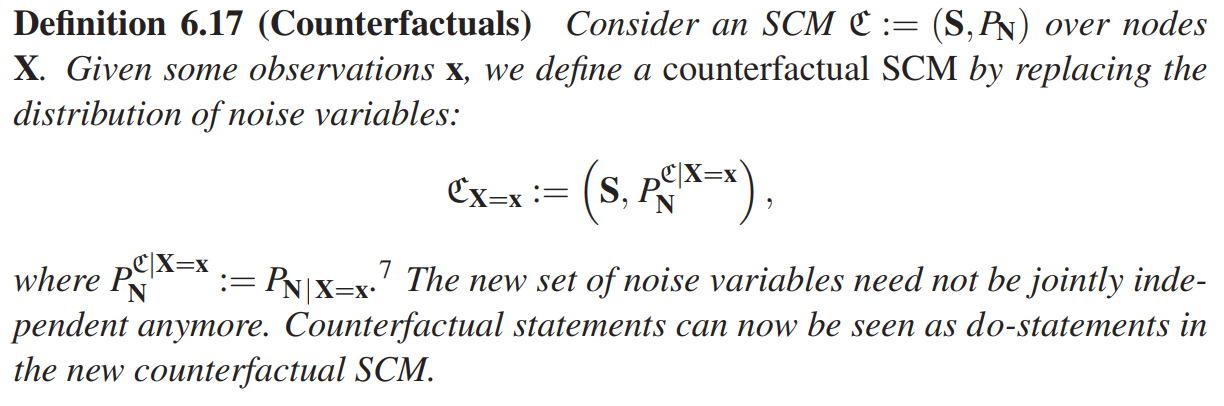
\includegraphics[scale=0.6]{fig22.png}}
    \begin{flushleft}
        Counterfactual corresponds to updating the noise distributions of an SCM (by conditioning) and then 
        performing an intervention.
    \end{flushleft}
\end{frame}

\begin{frame}
    \frametitle{Example}
    \leftline{Consider the SCM} 
    \centering{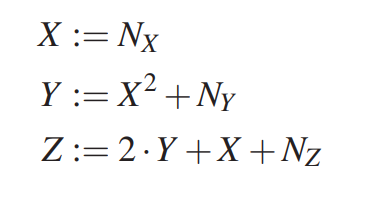
\includegraphics[scale=0.6]{fig23.png}} \\
    \begin{flushleft}
        with $N_x,N_y,N_z\overset{iid}\sim U(\{-5,-4,\cdots,4,5\})$. Assume that we observe $(X,Y,Z)=(1,2,4)$, then $Z$ would have
        been 11 had $X$ been set to 2.
    \end{flushleft}
    \centering{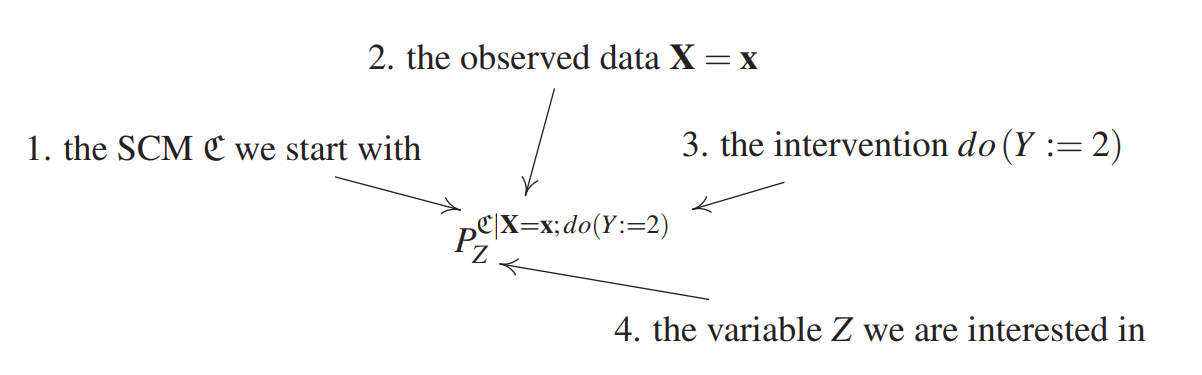
\includegraphics[scale=0.6]{fig24.png}}
\end{frame}

\begin{frame}
    \frametitle{Example}
    \begin{flushleft}
        This example shows two SCMs that induce the same graph, observational distributions,
        and intervention distributions but entail different counterfactual statements. 
    \end{flushleft} 
    \centering{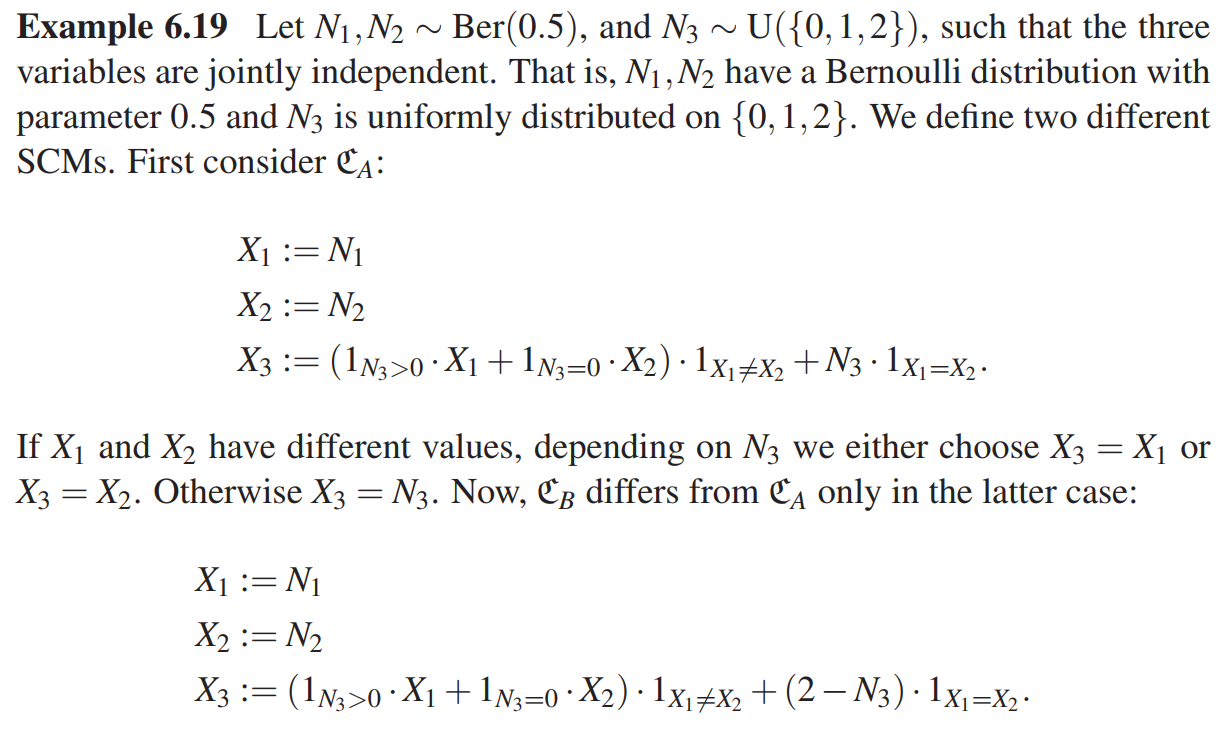
\includegraphics[scale=0.6]{fig25.png}}
\end{frame}

\section{Markov Property, Faithfulness, and Causal Minimality}

\begin{frame}
    \frametitle{Contents}
    \tableofcontents[currentsection]
\end{frame}

\begin{frame}
    \frametitle{Markov property} 
    \centering{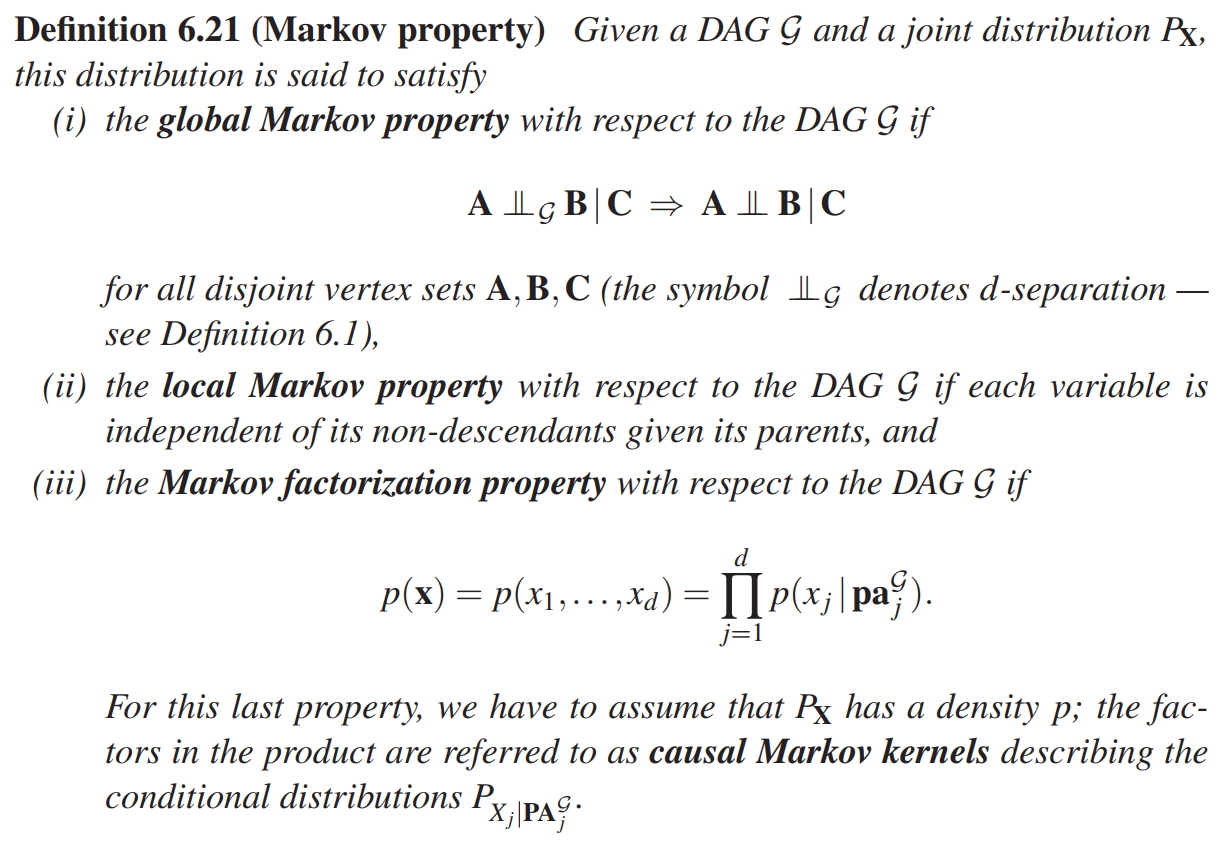
\includegraphics[scale=0.6]{fig26.png}}
    \centering{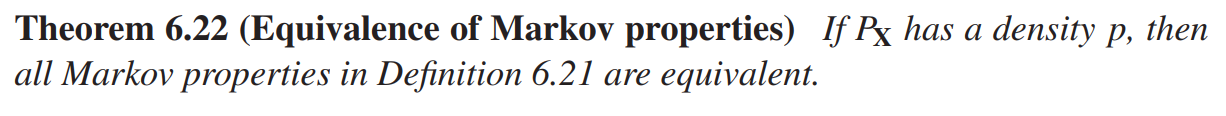
\includegraphics[scale=0.6]{fig27.png}}
\end{frame}

\begin{frame}
    \frametitle{Example} 
    \centering{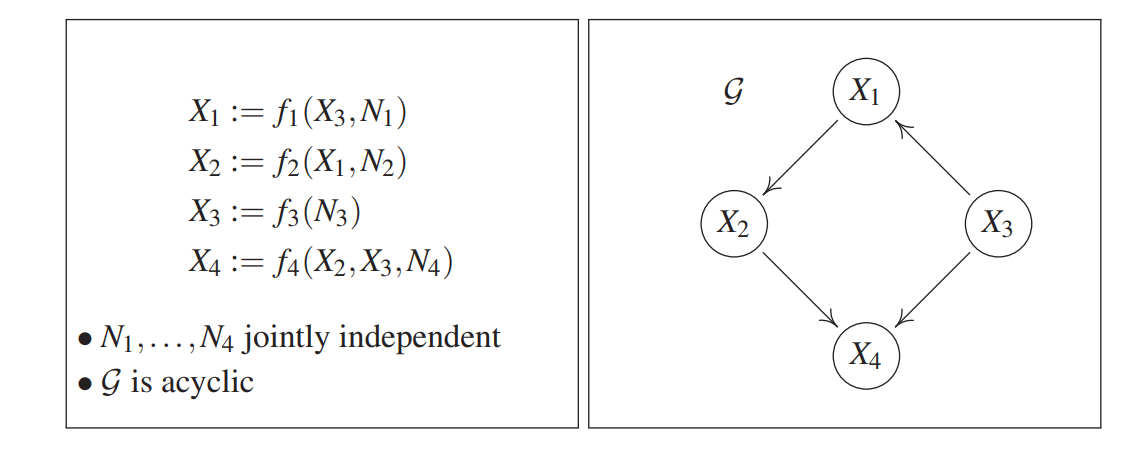
\includegraphics[scale=0.6]{fig5.png}}
    \begin{flushleft}
        The Markov condition relates statements about graph separation to conditional
        independences.
    \end{flushleft}
    \centering{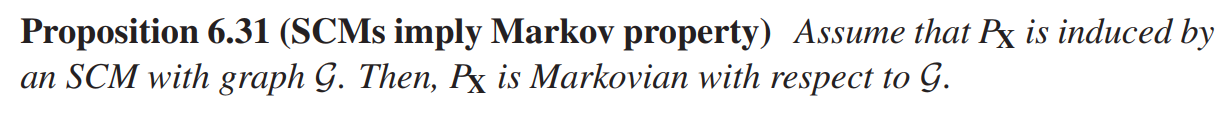
\includegraphics[scale=0.6]{fig35.png}}
\end{frame}

\begin{frame}
    \frametitle{Markov equivalence of graphs} 
    \begin{flushleft}
        Different graphs may encode the exact same set of conditional independences.
    \end{flushleft}
    \centering{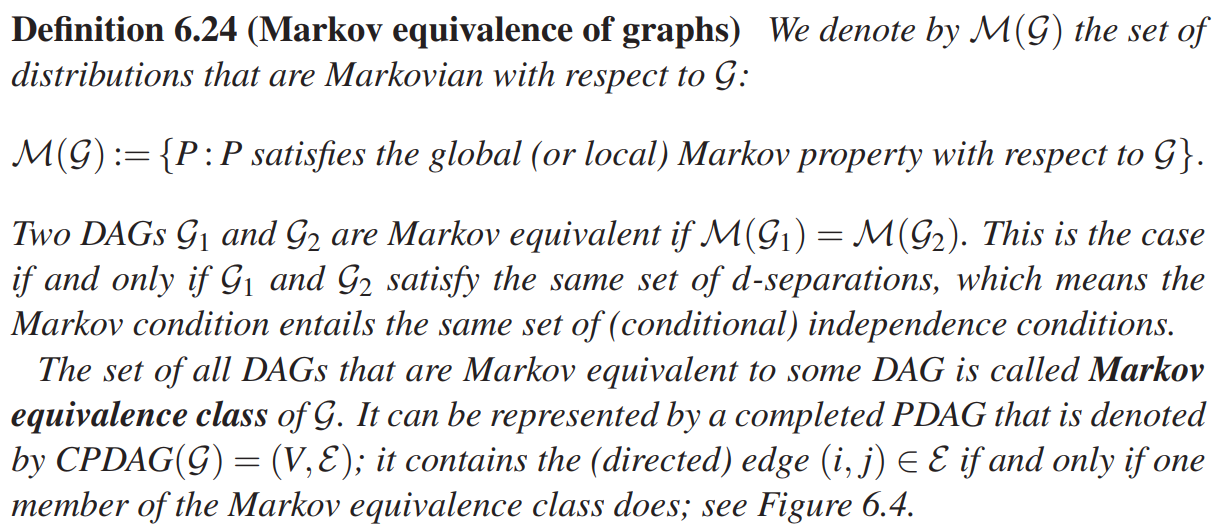
\includegraphics[scale=0.6]{fig28.png}}
\end{frame}

\begin{frame}
    \frametitle{Markov equivalence of graphs} 
    \centering{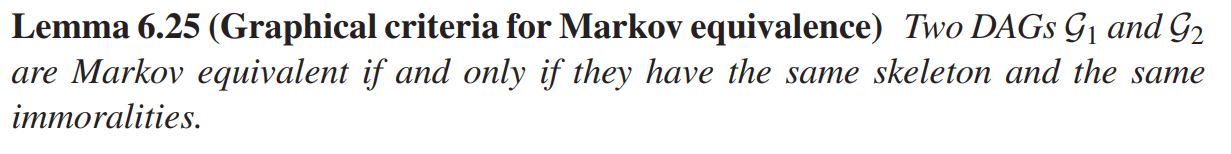
\includegraphics[scale=0.6]{fig29.png}}
    \centering{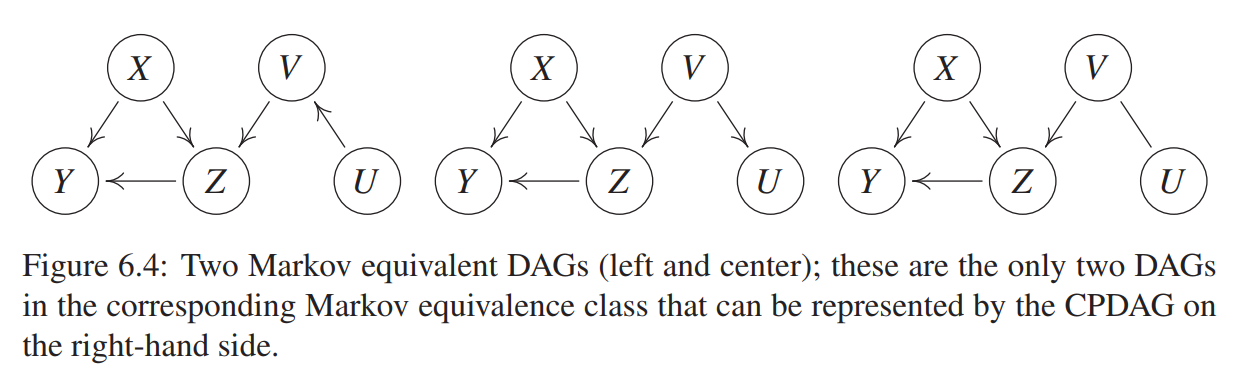
\includegraphics[scale=0.6]{fig30.png}}
\end{frame}

\begin{frame}
    \frametitle{Markov blanket} 
    \centering{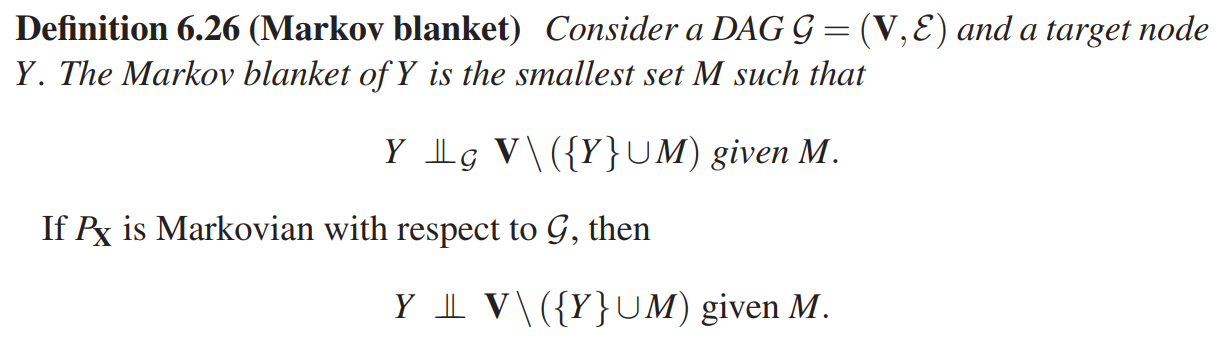
\includegraphics[scale=0.6]{fig31.png}}
    \begin{flushleft}
         In other words, given $M$, the other variables do not provide any further information about $Y$.
    \end{flushleft}
    \centering{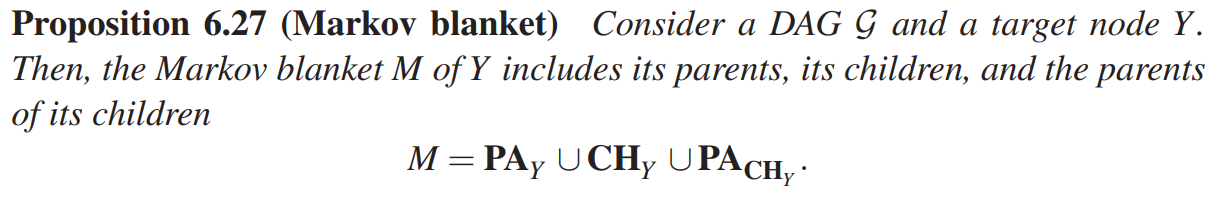
\includegraphics[scale=0.6]{fig32.png}}
\end{frame}

\begin{frame}
    \frametitle{Reichenbach's common cause principle}
    \begin{flushleft}
        Markov property relates distributions and graphs, then it can be used to justify Reichenbach's common cause principle.  
    \end{flushleft}
    \centering{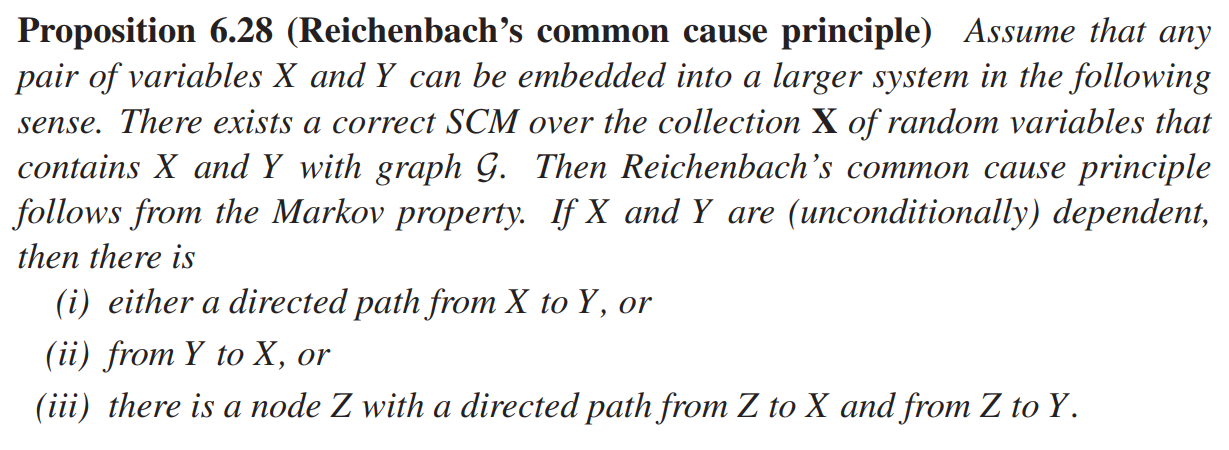
\includegraphics[scale=0.6]{fig33.png}}
\end{frame}

% \begin{frame}
%     \frametitle{Example: Berkson's paradox} 
%     Why are handsome men such jerks? \\
%     Let us assume that whether men are in a relationship($R=1$) is determined only by whether they are 
%     handsome ($H=1$) and whether they are friendly ($F=1$). More precisely, assume that the correct SCM has the form \\
%     \centering{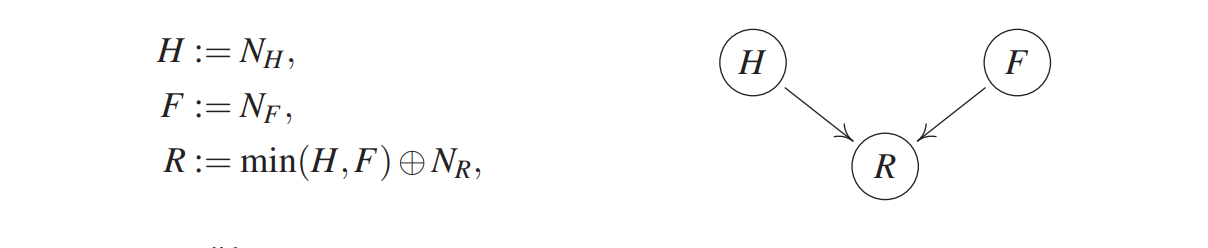
\includegraphics[scale=0.6]{fig34.png}} \\
%     \leftline{with $N_H,N_F\overset{iid}\sim Ber(0.5)$ and $N_R\sim Ber(0.1)$.}
% \end{frame}

% \begin{frame}
%     \frametitle{SCMs imply Markov property} 
%     \centering{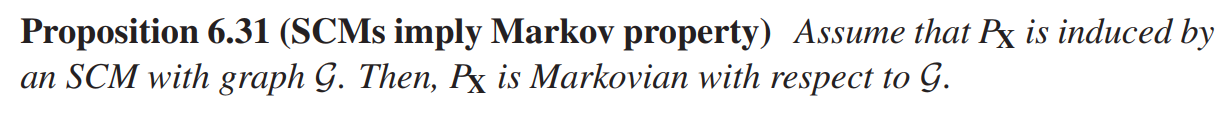
\includegraphics[scale=0.6]{fig35.png}}
% \end{frame}

\begin{frame}
    \frametitle{Causal graphical model} 
    \centering{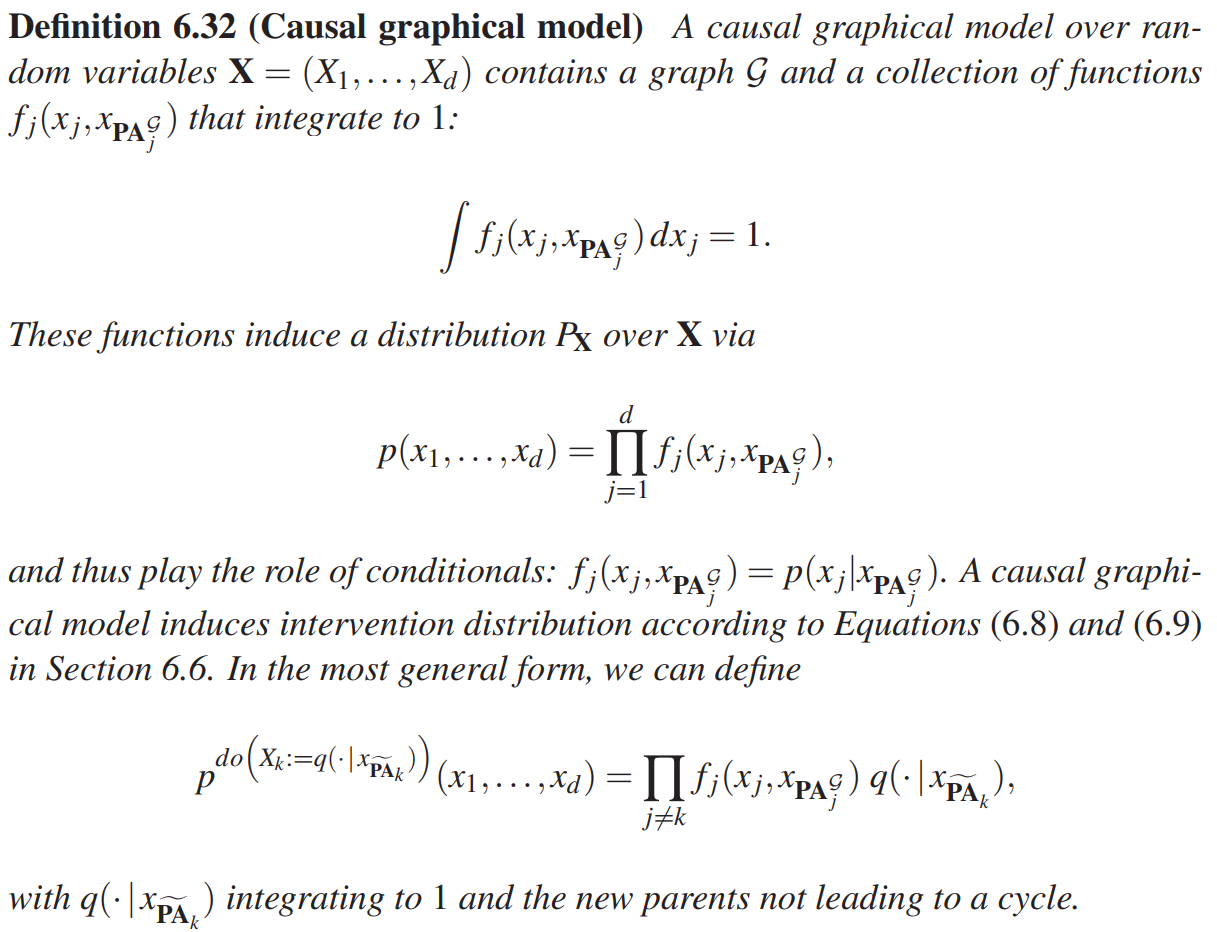
\includegraphics[scale=0.6]{fig36.png}}
\end{frame}

\begin{frame}
    \frametitle{Faithfulness and Causal Minimality}
    \begin{flushleft}
        Markov assumption enables us to read off independences from the graph structure. Faithfulness however, allows us to infer
        dependences from the graph structure. 
    \end{flushleft}
    \centering{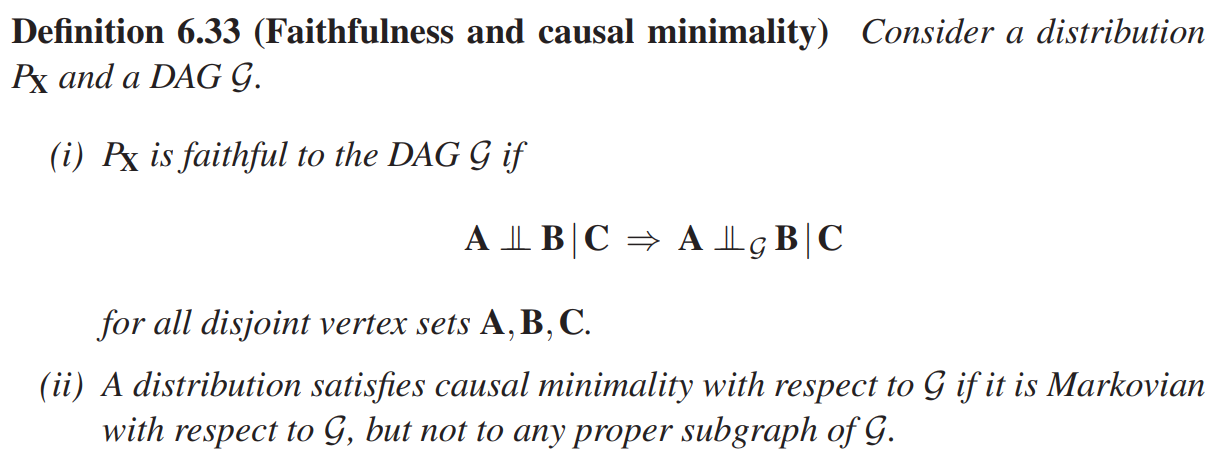
\includegraphics[scale=0.6]{fig37.png}}
\end{frame}

% \begin{frame}
%     \frametitle{Faithfulness and Causal Minimality}
%     \centering{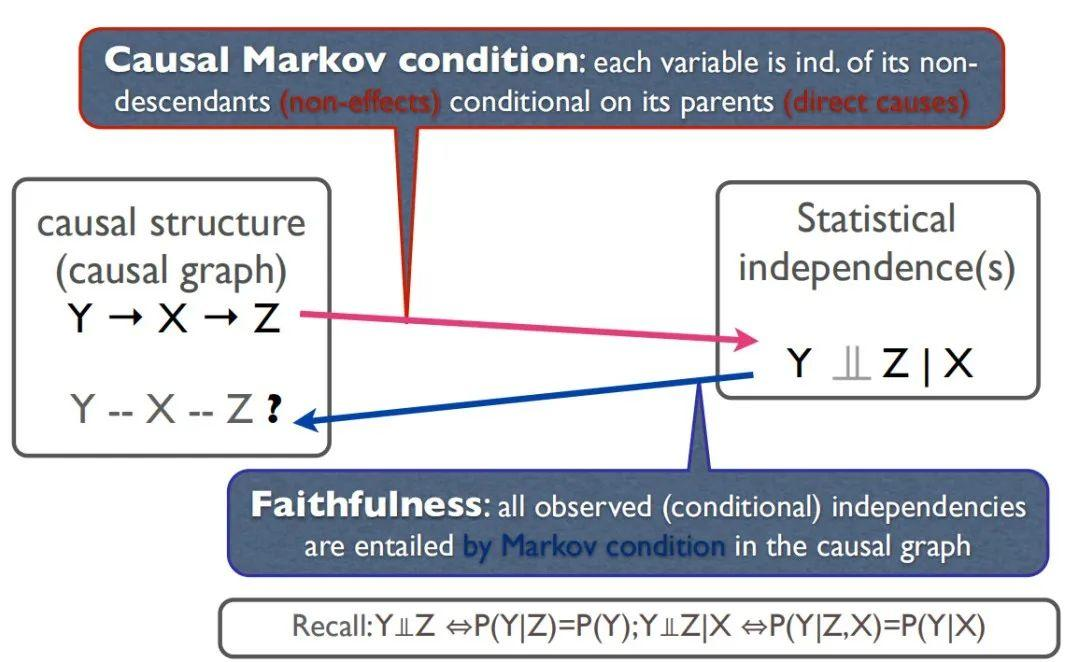
\includegraphics[scale=0.25]{fig42.jpeg}}
% \end{frame}

\begin{frame}
    \frametitle{Example} 
    \centering{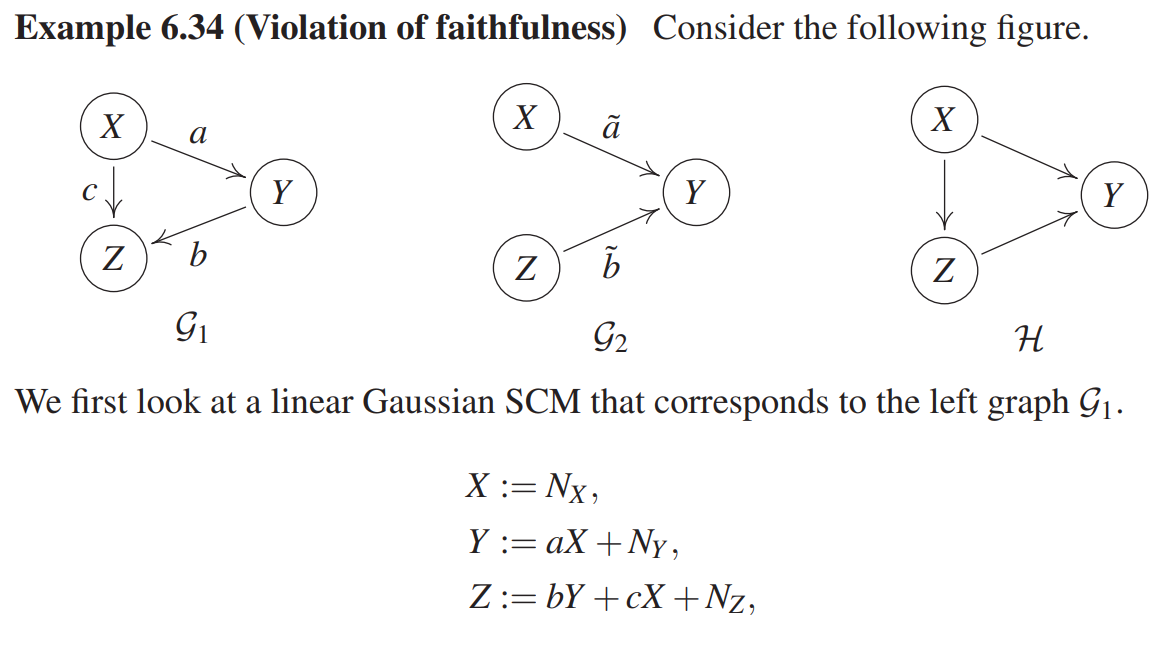
\includegraphics[scale=0.6]{fig38.png}}
    \begin{flushleft}
        If $ab+c=0$, the distribution is not faithful with respect to $\mathcal{G}_1$ since we obtain $X\Vbar Z$, which is
        not implied by the graph structure.
    \end{flushleft}
\end{frame}

\begin{frame}
    \frametitle{Faithfulness and causal minimality} 
    \centering{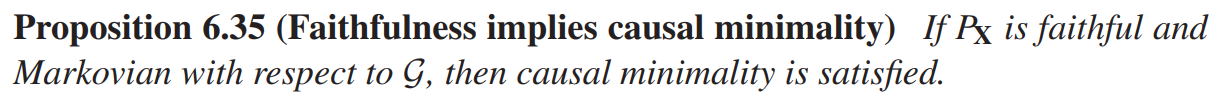
\includegraphics[scale=0.6]{fig39.png}}
    \begin{flushleft}
        A distribution is minimal with respect to $\mathcal{G}$ if and only if there is no node that is conditionally 
        independent of any of its parents, given the remaining parents.
    \end{flushleft}
    \centering{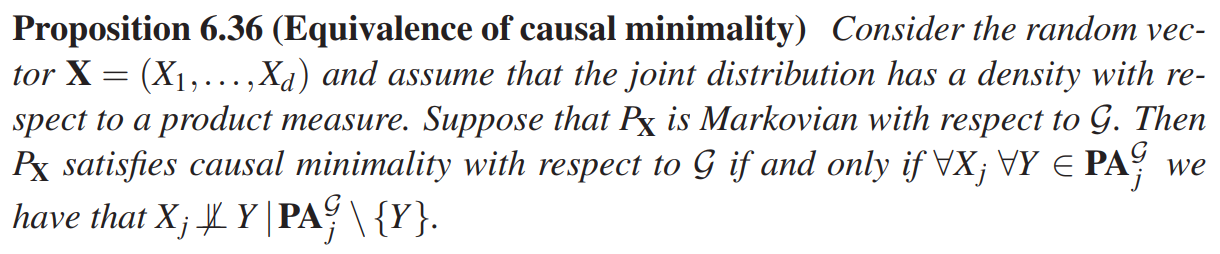
\includegraphics[scale=0.6]{fig40.png}}
\end{frame}

\begin{frame}
    \frametitle{Reference} 
    Pearl J, Glymour M, Jewell N P. Causal inference in statistics: A primer[M]. John Wiley \& Sons, 2016. \\
    Murphy K P. Machine learning: a probabilistic perspective[M]. MIT press, 2012. \\
\end{frame}


\end{document}
